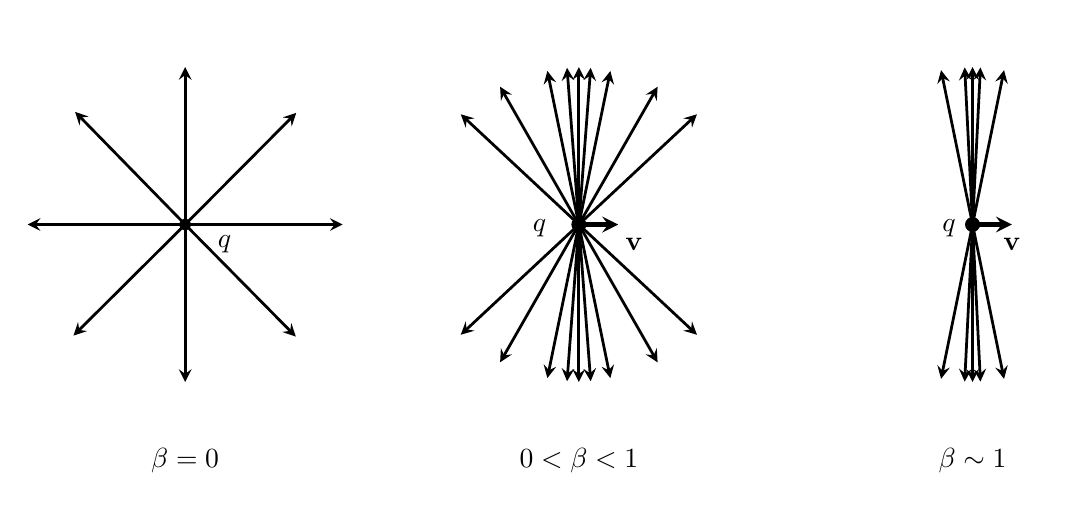
\begin{tikzpicture}[line cap=round,line join=round,>=stealth,x=1cm,y=1cm]
\clip(-2.,-3.5) rectangle (11,2.5);
\draw [->,line width=1pt] (0,0) -- (-1.3975053304790308,1.4307266864368944);
\draw [->,line width=1pt] (0,0) -- (0,2);
\draw [->,line width=1pt] (0,0) -- (1.41035916900663,1.4180574792295721);
\draw [->,line width=1pt] (0,0) -- (2,0);
\draw [->,line width=1pt] (0,0) -- (1.4051129272120964,-1.4232560071123728);
\draw [->,line width=1pt] (0,0) -- (0,-2);
\draw [->,line width=1pt] (0,0) -- (-1.4180074832552354,-1.4104094360972468);
\draw [->,line width=1pt] (0,0) -- (-2,0);

\draw [->,line width=1pt] (5,0) -- (3.5,1.4);
\draw [->,line width=1pt] (5,0) -- (6.5,1.4);
\draw [->,line width=1pt] (5,0) -- (3.5,-1.4);
\draw [->,line width=1pt] (5,0) -- (6.5,-1.4);
\draw [->,line width=1pt] (5,0) -- (5,2);
\draw [->,line width=1pt] (5,0) -- (5,-2);
\draw [->,line width=1pt] (5,0) -- (4.6,-1.95);
\draw [->,line width=1pt] (5,0) -- (5.4,-1.95);
\draw [->,line width=1pt] (5,0) -- (4.6,1.95);
\draw [->,line width=1pt] (5,0) -- (5.4,1.95);

\draw [->,line width=1pt] (5,0) -- (4.85,-1.99);
\draw [->,line width=1pt] (5,0) -- (5.15,-1.99);
\draw [->,line width=1pt] (5,0) -- (4.85,1.99);
\draw [->,line width=1pt] (5,0) -- (5.15,1.99);

\draw [->,line width=1pt] (5,0) -- (6.,1.75);
\draw [->,line width=1pt] (5,0) -- (4.,1.75);
\draw [->,line width=1pt] (5,0) -- (4.,-1.75);
\draw [->,line width=1pt] (5,0) -- (6.,-1.75);


\draw [->,line width=1pt] (10,0) -- (10,2);
\draw [->,line width=1pt] (10,0) -- (10,-2);
\draw [->,line width=1pt] (10,0) -- (10.4,1.96);
\draw [->,line width=1pt] (10,0) -- (9.6,-1.96);
\draw [->,line width=1pt] (10,0) -- (10.1,1.995);
\draw [->,line width=1pt] (10,0) -- (9.9,1.995);
\draw [->,line width=1pt] (10,0) -- (9.9,-1.995);
\draw [->,line width=1pt] (10,0) -- (10.1,-1.995);
\draw [->,line width=1pt] (10,0) -- (9.6,1.96);
\draw [->,line width=1pt] (10,0) -- (10.4,-1.96);

\draw (0,-3) node[anchor=center] {$\beta =0$};
\draw (5, -3) node[anchor=center] {$ 0 < \beta < 1$};
\draw (10,-3) node[anchor=center] {$\beta \sim 1$};

\draw (0.5,-0.25) node[anchor=center] {$q$};
\draw (4.5,-0.05) node[anchor=center] {$q$};
\draw (9.7,-0.05) node[anchor=center] {$q$};

\draw [->,line width=1.5pt] (10,0) -- (10.5,0);
\draw (10.5, -0.25) node[anchor=center] {$\mathbf{v}$};
\draw [->,line width=1.5pt] (5,0) -- (5.5,0);
\draw (5.7, -0.25) node[anchor=center] {$\mathbf{v}$};



\begin{scriptsize}
\draw [fill=black] (0,0) circle (2pt);
\draw [fill=black] (10,0) circle (2.5pt);
\draw [fill=black] (5,0) circle (2.5pt);
\end{scriptsize}

\end{tikzpicture}